\chapter{System description}
This chapter covers the design and implementation of SemReBot2, a system architecture that enables a robot to gain semantic knowledge in natural language. It begins with a brief overview of the architecture before describing each module, including the simulation environment. The chapter ends with a deeper study of the modules and the data pipeline. See Appendix \textcolor{red}{X} for a video demo\footnote{As of April 24th 2024, the software packages used in SemReBot2 is migrating to Ubuntu 24.04. This creates dependency issues related to the simulation environment and graphical user interface\cite{stinkyelias_source_2024}. Therefore, the video demo is showing a terminal-like simulation environment instead of a 3D world.}.

SemReBot2 is specialized in a pick-and-place scenario of pallets in a simulated warehouse. The goal is to allow humans interfere with robots by using their voice only, which makes robots available for everyone that can speak. 

\section{SemReBot2 overview}
An overview of the SemReBot2 pipeline is shown in Figure \ref{fig:semrebot2_overview}. Based on human speech, SemReBot2 translates this speech into suitable actions that a robot can perform. SemReBot2 inputs natural language speech, $u_{s}$, and transforms it to natural language text, $u_{t}$, with ASR. An LLM generates PDDL problem instances $\mathbf{P}_{i}$, predicates $\mathbf{P}_{p}$ and goals $\mathbf{P}_{g}$, passed to PlanSys2 for evaluation. An AI planner within PlanSys2 generates a plan $\mathbf{P}_{plan}$ with corresponding actions $\mathbf{a}$ that a robot can execute in the physical world.

\begin{figure}[h]
    \centering
    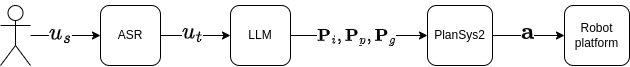
\includegraphics[width=\textwidth]{figures/overview_semrebot2.png}
    \caption[SemReBot2 overview]{Overview of SemReBot2 pipeline. There are no feedback loops in the pipeline.}
    \label{fig:semrebot2_overview}
\end{figure}

SemReBot2 leverages three main open source projects wrapped in ROS 2 to function: OpenAI's Whisper ASR model for speech-to-text tasks, MistralAI's Mistral 7B Instruct LLM for semantic reasoning, and PlanSys2, a PDDL-based planning system implemented in ROS 2.

\section{SemReBot2 modules}
SemReBot2 uses ROS 2 to combine the different components to run on a robotics platform.

\subsection{Automatic speech recognition module}
The first module in the data pipeline is the ASR module. The ASR module is the only module that directly interferes with a human by converting speech to text. The conversion is done by the large Whisper model. Whisper can be combined with ROS 2 through Hugging Face's transformers library in Python which also allows the user to load the model to a GPU with flash attention. The loading of the model with flash attention decreases the inference time (see Section \ref{sec:Whisper_experiments}) which we count as an important metric in a real-time robotics system.

In SemReBot2, automatic speech recognition is handled by the ROS 2 lifecycle node \newline\verb|whisper_lifecycle_node|. Figure \ref{fig:whisper_lifecycle} shows a simplified state diagram. Choosing it as a lifecycle node allows a fail-safe mechanism in case memory has to be freed or reallocated during runtime. It is also convenient during testing to isolate modules with managed state transitions.

\begin{figure}[h]
    \centering
    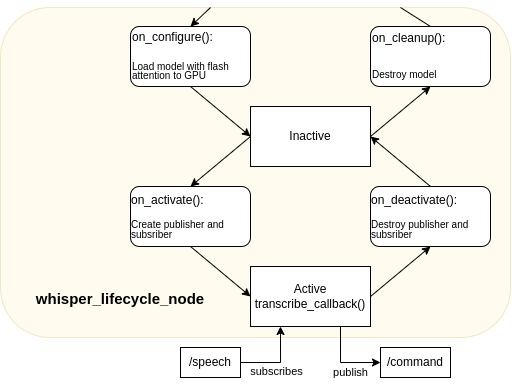
\includegraphics[width=0.8\textwidth]{figures/whisper_lifecycle.png}
    \caption[Whisper lifecycle node]{A simple state diagram of Whisper lifecycle node.}
    \label{fig:whisper_lifecycle}
\end{figure}

Upon activation, Whisper have been loaded to a GPU and the node is subscribing to the topic \verb|/speech|. Once a message is received, the \verb|transcribe_callback| method is called and the incoming audio $u_{s}$ is transcribed before it publishes $u_{t}$ as a \verb|std_msgs/msg/String| on the \verb|/command| topic. Until a new message is received, our Whisper node is on standby.

\subsection{Large language model module}
The large language model module boasts the same skeleton design as \verb|whisper_lifecycle_node|. It is a managed lifecycle node running Mistral 7B model in 4-bit quantized size. Again, Hugging Face's transformers library lets us load the model in a Python script and use it with ROS 2. The \verb|BitsAndBytesConfig| class allows us to load the model in 4-bit, which greatly reduces memory allocation (although at the cost of performance) compared to the full precision model.

\begin{figure}[ht]
    \centering
    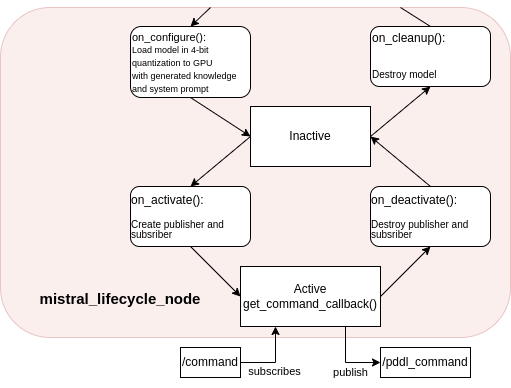
\includegraphics[width=0.8\textwidth]{figures/mistral_lifecycle.png}
    \caption[Mistral lifecycle node]{A simple state diagram of the Mistral lifecycle node.}
    \label{fig:mistral_lifecycle}
\end{figure}

When transitioning \verb|mistral_lifecycle_node| to a configured state, Mistral is loaded to the GPU with generated knowledge and a system prompt. The generated knowledge and system prompt is necessary in order to instruct Mistral to respond to commands in the desired format. The system prompt explains that Mistral is running on an AGV forklift as a "PDDL assistant". It also contains the necessary info from \verb|domain.pddl| such as the different types that is allowed and the possible predicates. Functions and actions are excluded, as they have no value for the language model.
Generated knowledge contains instances and predicates that are true at all times. That is, for example, the robot exists and the zones inside the warehouse have shelves or a charging station.

When the node's callback function is called, Mistral is few-shot prompted with ten examples to guide Mistral to answer in a certain way. A shot is designed to tell Mistral "given \textit{this} domain and command, output in \textit{this} format".

\begin{figure}[ht]
    \centering
    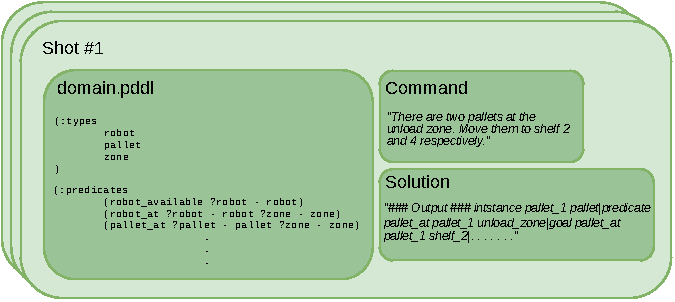
\includegraphics[width=\textwidth]{figures/few-shot_prompting.pdf}
    \caption[Few-shot prompting]{An example shot prompted to Mistral with the solution output, given a domain and command.}
    \label{fig:few_shot_prompt_mistral}
\end{figure}

The output format is designed in such a way that it can be passed to PlanSys2's client API (see Section \ref{ssec:semrebot2_task_controller}) with simple string parsing. The output format always begin with a prompt guard \verb|### Output ###| and ends with an end token "|". In this manner, any tokens generated by Mistral preceding the prompt guard and following the final end token can be discarded before passed to PlanSys2's client API by publishing a \verb|std_msgs/msg/String| to the \verb|/pddl_command| topic.

To keep the input memory at the same size as commands are given to Mistral, the previous command and output is discarded. The system prompt, generated knowledge, and the ten shots are all passed to the model for every inference call, which makes the allocated memory nearly steady.

\subsection{Task controller}\label{ssec:semrebot2_task_controller}
SemReBot2 interacts with PlanSys2 by running a node \verb|task_controller| as a client application to PlanSys2. With PlanSys2's client API, the \verb|task_controller| can interact with the \verb|Executor|, \verb|Planner|, \verb|Domain Expert| and \verb|Problem Expert| in PlanSys2 through shared pointers.

The Task controller receives the same generated knowledge as Mistral, and by initialization, it sends the generated knowledge including function values of robot speed, battery level and distances between zones to the \verb|Problem Expert|.

The node's callback function is called once a message on the topic \verb|/pddl_command| is published. This message is parsed and additional instances and predicates, as well as one or more goals, are sent to the \verb|Problem Expert|. Further, Task controller invokes the \verb|Problem Expert| and \verb|Domain Expert| to redirect the problem and domain to the \verb|Planner|, which creates a plan with the POPF plugin. If the plan from the \verb|Planner| is valid, Task controller invokes the \verb|Executor| to execute the plan by first building the BT trees necessary and then tick each BT node in correct order.

\begin{algorithm}\label{alg:task_controller}
\caption{Task Controller Node}
    \begin{algorithmic}[1]
        \State Add generated knowledge to problem\_expert
        \Procedure{task\_callback}{message}
            \For{parsed instance, predicate, goal \textbf{in} message}
                \State Add instance, predicate, goal to problem\_expert
            \EndFor
            \State domain := getDomain()
            \State problem := getProblem()
            \State plan := getPlan(domain, problem)
            \If{plan has value}
                \State Execute plan
            \EndIf
        \EndProcedure
    \end{algorithmic}
\end{algorithm}

\subsection{Custom behavior tree nodes}\label{ssec:custom_behavior_tree_nodes}
BT nodes represent the logic of robotic actions. We created six custom BT action nodes to simulate the necessary actions to pick up and place one or more pallets. The custom BT nodes are \verb|ApproachPallet|, \verb|LeavePallet|, \verb|LowerFork|, \verb|RaiseFork|, \verb|Navigate| and \verb|Recharge|, which can be combined into three BTs \verb|Navigate|, \verb|Transport| and \verb|Recharge|, that the BT builder can combine according to the provided plan from POPF.

Using the custom \verb|Navigate| BT node as an example, it is responsible for sending goal poses to Nav2's \verb|NavigateToPose| action based on a plan. SemReBot2 launches a ROS 2 node \newline\verb|navigate_cmd| which is an instance of PlanSys2's BTAction, which again is a BT action node. \verb|navigate_cmd| include parameters such as the waypoints in the warehouse and the XML schema of the \verb|Navigate| BT node.

\begin{lstlisting}[language=XML, caption=The custom BT node Navigate, label=lst:navigate_xml]
<root BTCPP_format="4" main_tree_to_execute = "MainTree">
    <BehaviorTree ID="MainTree">
        <Sequence name="root_sequence">
            <Navigate name="navigate" goal="{arg2}"/>
        </Sequence>
    </BehaviorTree>
</root>
\end{lstlisting}

When the BTAction node \verb|navigate_cmd| is activated, it creates the BT from the XML schema, Listing \ref{lst:navigate_xml}, and initialises a blackboard with ports including a shared pointer to a ROS 2 node and a goal pose. The goal pose is inserted to the blackboard by the Executor's BT builder in PlanSys2 and uses the \verb|?to-zone| parameter from the \verb|navigate| durative action in the PDDL plan (not to be mistaken by the \verb|Navigate| BT node or \verb|navigate_cmd| ROS node.

\begin{lstlisting}[caption={The PDDL action navigate's parameters}, label=lst:navigate_pddl]
(:durative-action navigate
    :parameters (?robot - robot ?from_zone - zone ?to_zone - zone)
\end{lstlisting}

When our custom BT node \verb|Navigate| is constructed, it retrieves the shared pointer to the ROS node \verb|navigate_cmd| and the goal from the PDDL plan from the blackboard. The shared pointer allows the \verb|Navigate| BT node to access the ROS parameters, which include the waypoint coordinates. When the \verb|Navigate| BT node is ticked, it checks the value in the key-value pair \verb|goal| in the blackboard and sends the corresponding coordinate as a goal to the \verb|NavigateToPose| action server, which is a part of the Nav2 navigation stack.

\subsection{Lifecycle manager}
As with Nav2 and PlanSys2, SemReBot2 has a lifecycle manager to manage the lifecycle transition states for \verb|whisper_lifecycle_node| and \verb|mistral_lifecycle_node|. When launching the bringup launch file for SemReBot2, Whisper and Mistral lifecycle nodes are launched in an unconfigured state together with the lifecycle manager, among others. The lifecycle manager transitions the two nodes between states in a single-threaded executor as Whisper and Mistral works sequentially.

\begin{algorithm}\label{alg:lifecycle_manager}
    \caption{Lifecycle Manager}
    \begin{algorithmic}[1]
        \Procedure{Main}{}
            \State Create LifecycleManager for "whisper" and "mistral"
            \State Init SingleThreadedExecutor
            \For{each node in manager\_nodes}
                \State Init node
                \State Add node to executor
            \EndFor
            \State Asynchronous startup function with 30 seconds timeout
            \State Spin executor until startup function is complete
            \If{startup failed}
                \State Log error and shutdown
                \State \Return -1
            \EndIf
            \State Shutdown
            \State \Return 0
        \EndProcedure
    \end{algorithmic}
\end{algorithm}

The lifecycle manager uses service calls to ROS 2's \verb|lifecycle_msgs| services through its API. This is handled by the \verb|startup_function| method which brings the lifecycle nodes from an unconfigured state to an active state.

Algorithm \ref{alg:lc_mngr_startup} is simple, yet crucial. For every transition service call, Whisper and Mistral calls their \verb|on_configure()| and \verb|on_activate()| methods. See Figures \ref{fig:whisper_lifecycle} and \ref{fig:mistral_lifecycle}. The lifecycle manager allows for a controlled and automated startup and shutdown of lifecycle nodes.

\begin{algorithm}\label{alg:lc_mngr_startup}
\caption{Lifecycle managers simplified startup procedure}
    \begin{algorithmic}[1]
        \Function{startup\_function}{manager\_nodes, timeout}
            \For{node \textbf{in} [whisper, mistral]}
                \State transition node to INACTIVE
            \EndFor
            \For{node \textbf{in} [whisper, mistral]}
                \State transition node to ACTIVE
            \EndFor
        \EndFunction
    \end{algorithmic}
\end{algorithm}

\section{Simulation environment}
Without a physical robot, we have to run SemReBot2 in a simulated environment. There are several simulators to choose from, but to avoid extending the scope of this thesis, we use the Gazebo Classic simulator with the standard empty world and Turtlebot3 as our robot.

\begin{figure}[ht]
    \centering
    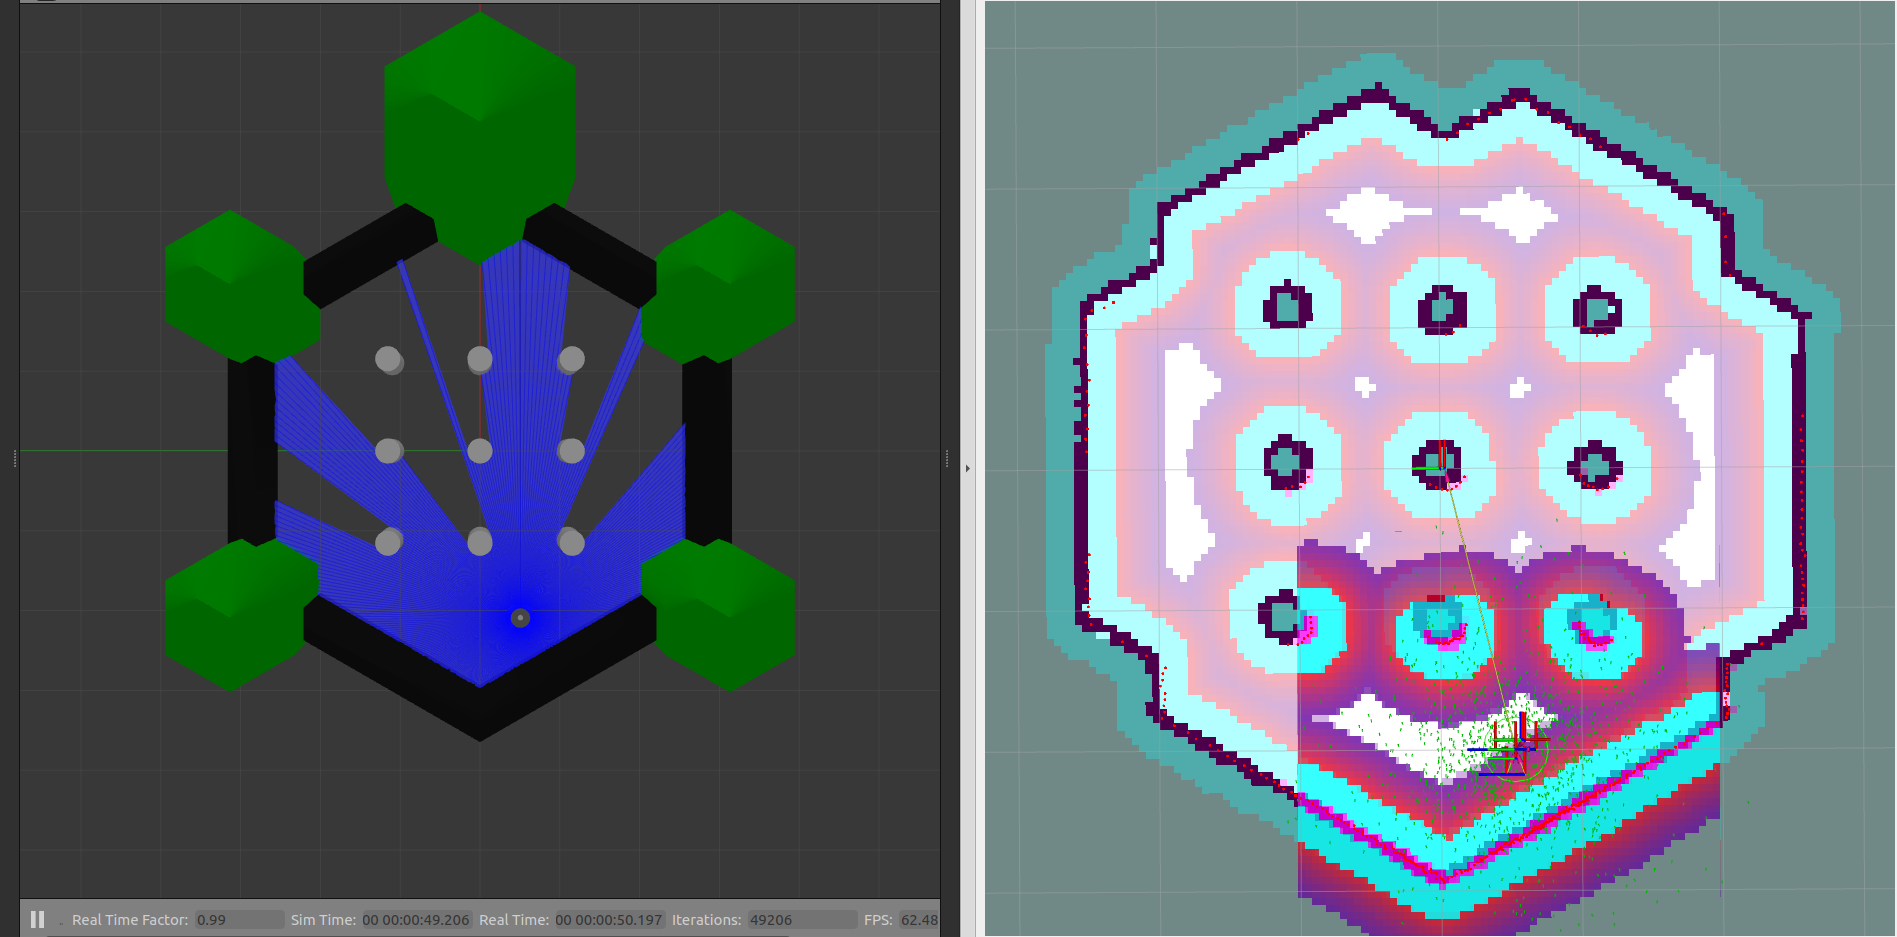
\includegraphics[width=\textwidth]{figures/screenshot_sim_world.png}
    \caption[Simulation environment]{Screenshot of Turtlebot3 in Gazebo (left) and RViz2 (right).}
    \label{fig:screenshot_simworld}
\end{figure}

Using Turtlebot3 means that we have no AGV forklift and, therefore, no direct implementation of the fork and its pick-and-place actions. Instead, these actions are simulated with behaviour tree nodes, as explained in Section \ref{ssec:custom_behavior_tree_nodes}. Lastly, the environment is simulated as a warehouse. A warehouse usually consists of shelves for pallets and goods, one or several loading docks, and charging stations for electric forklifts and/or AGVs. Our environment simulates such zones by passing coordinates of a hypothetical charging station, unload zone and four shelves to SemReBot2. 

\begin{figure}
    \centering
    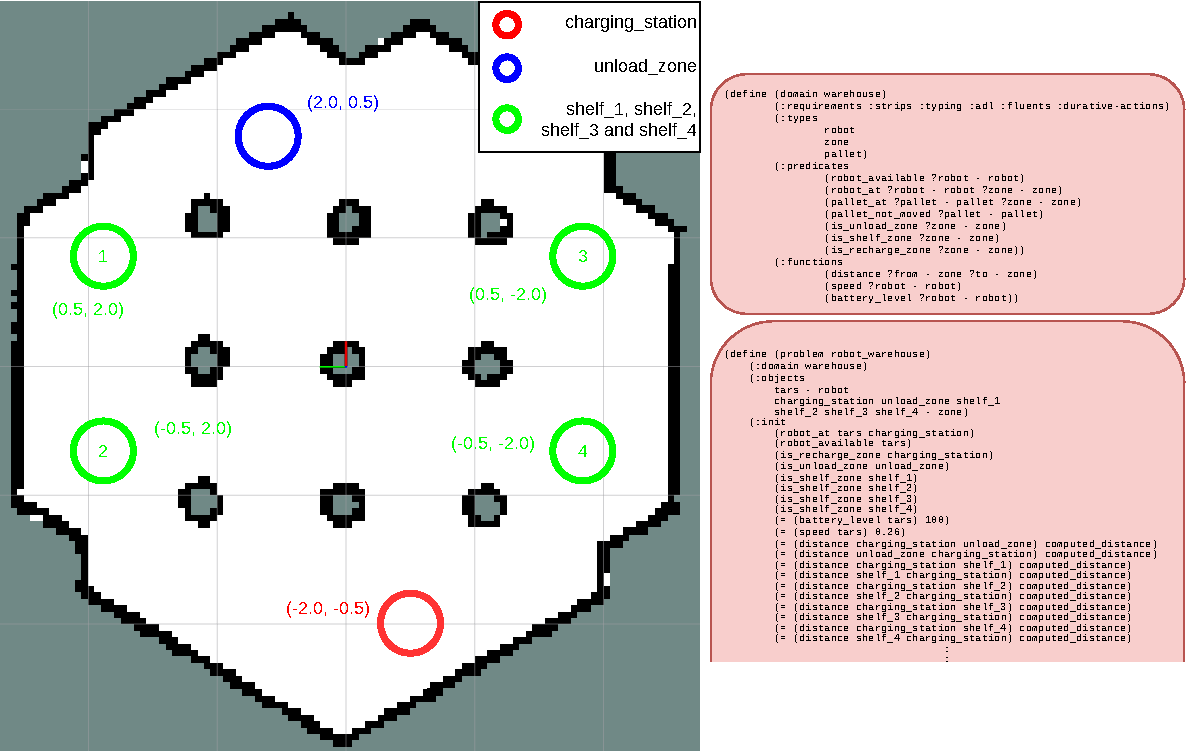
\includegraphics[width=0.8\textwidth]{figures/combined_domain.pdf}
    \caption[Simulated world knowledge]{A map of the different zones with correpsonding 2D coordinates (left) and domain and problem knowledge fed to SemReBot2 and PlanSys2 (right).}
    \label{fig:sim_world_knowledge}
\end{figure}

Turtlebot3 uses simulated LiDAR and odometry data for navigation, but neither SemReBot2 nor PlanSys2 receives data from sensors. Instead, they receive information about the physical/simulated world from a provided \verb|domain.pddl| file and voice commands processed by Whisper node and Mistral node. In addition, Task controller node's constructor is passing constant initial knowledge to PlanSys2, such as robot and zones instances and function values like battery level and distance between the zones. Sensor data is handled by Nav2, receiving waypoints to navigate to and goal poses from the Navigate BT node, which again is ticked by the Executor in PlanSys2.

For detailed information on plugins used in Nav2 and Gazebo, see Appendix \textcolor{red}{X}.

\section{Detailed}
This section will provide a detailed example of how SemReBot2 works in conjunction with PlanSys2, Nav2, and Turtlebot3. We provide an example at each step so the reader can follow along how speech is converted to robot actions. It can be divided into several steps.

\begin{figure}
    \centering
    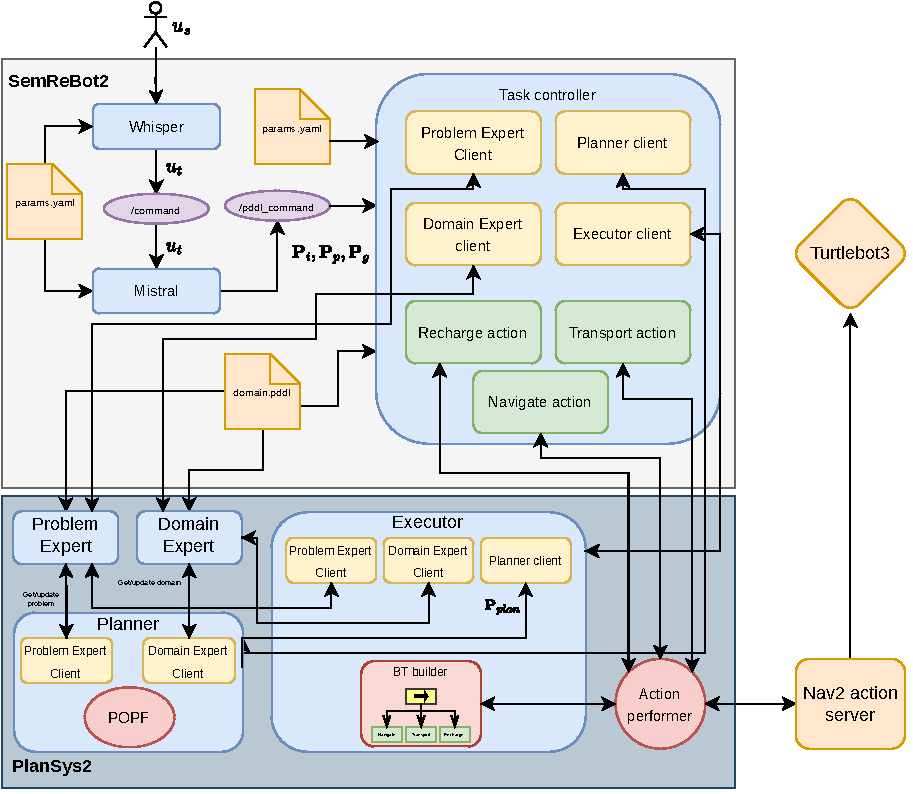
\includegraphics[width=0.8\textwidth]{figures/semrebot2.pdf}
    \caption[SemReBot2 detailed overview]{Detailed overview of data flow in SemReBot2 and PlanSys2 with Nav2 and Turtlebot3}
    \label{fig:semrebot2}
\end{figure}

\subsection{Step 1 - Speech-to-text}
When SemReBot2 is activated and a human is speaking, the audio stream $u_{s}$ is recorded mono with a sample rate of 16 kHz and 512 frames per buffer. The frames are concatinated to a single bytes object before its passed to Whisper as a \verb|NumPy| array of 16-bit integers. To decrease the inference time on Whisper, we transcribe $u_{s}$ with a chunk length of 30 seconds and a batch size of 24 chunks.

The first part of SemReBot2 can therefore be seen as a function that converts an audio signal into a sequence of words

\begin{equation}
    \label{eq:whisper_function}
    u_{t}=f(u_{s})
\end{equation}

\begin{example}\label{ex:whisper}
    Given the warehouse environment in Figure \ref{fig:sim_world_knowledge}, our robot TARS, an AGV forklift, is placed besides shelf 1 with 50\% battery capacity. A worker gives the command by voice

    \textit{TARS, move pallet number 1 from the unload zone to shelf number 1, and relocate pallet number 2 from the unload zone to shelf number 4.}

    SemReBot2 will recognise its being talked to and the command will be transcribed by Whisper, and published to the \verb|/command| topic.
\end{example}

\subsection{Step 2 - Create instances, predicates and goals}
Mistral receives the transcribed text $u_{t}$ and analyzes the semantics. Given the generated knowledge, system prompt and few-shot prompts, Mistral has learned how to output the correct instances, predicates and goals. They will be formatted into a single string and published to the \verb|/pddl_command| topic for further computation.

\begin{example}\label{ex:mistral}
    Continuing from Example \ref{ex:whisper}, Mistral extracts the necessary instances, predicates and goals from $u_{t}$ in the same format as defined in \verb|domain.pddl|:

    \begin{equation}
        \mathbf{P}_{i}=
        \begin{pmatrix}
            \text{p}_{1} \text{ pallet} \\
            \text{p}_{2} \text{ pallet}
        \end{pmatrix}
    \end{equation}
    
    \begin{equation}
        \mathbf{P}_{p}=
        \begin{pmatrix}
            \text{pallet\_at p}_{1} \text{ unload\_zone} \\    
            \text{pallet\_at p}_{2} \text{ unload\_zone} \\
            \text{pallet\_not\_moved p}_{1} \\
            \text{pallet\_not\_moved p}_{2}
        \end{pmatrix}
    \end{equation}

    \begin{equation}
        \mathbf{P}_{g} =
        \begin{pmatrix}
            \text{pallet\_at p}_{1} \text{ shelf\_1} \\
            \text{pallet\_at p}_{2} \text{ shelf\_4}
        \end{pmatrix}
    \end{equation}

Note that the predicates \verb|robot_at| and \verb|robot_available| is not used by Mistral due to the generated knowledge.
\end{example}

\subsection{Step 3 - Generate a PDDL plan}
The third step in SemReBot2 involves activating PlanSys2. The Task controller receives the instances, predicates and goals from Mistral, checks if they are eligible based on \verb|domain.pddl|, and passes them to the \verb|Planner|, \verb|Executor|, \verb|Problem Expert| and \verb|Domain Expert| through service calls.

\begin{example}\label{ex:task_controller}
    Continuing from Example \ref{ex:mistral}, the Task controller parses $\mathbf{P}_{i}$, $\mathbf{P}_{p}$ and $\mathbf{P}_{g}$ and make service calls to the \verb|Problem Expert| which adds the new knowledge to the \verb|problem.pddl| file.

    \begin{lstlisting}[caption={Parts of the problem file available for POPF. Only showing the added objects and initial knowledge received from Task controller.}, label=lst:ex_problem.pddl]
        (:objects
                :
            p1 p2 - pallet)
        (:init
                :
                :
            (pallet_at p1 unload_zone)
            (pallet_at p2 unload_zone)
            (pallet_not_moved p1)
            (pallet_not_moved p2))
        (:goal (and
            (pallet_at p1 shelf_1)
            (pallet_at p2 shelf_4)))
    \end{lstlisting}

    The \verb|Planner| receives the domain and problem file from the \verb|Problem Expert| and \newline\verb|Domain Expert| and makes a call to the POPF plugin, which generates the following plan:

    \begin{verbatim}
        0:      (navigate tars shelf_1 charging_station)      [13.598]
        13.599:	(recharge tars charging_station)              [10]
        23.6:   (navigate tars charging_station unload_zone)  [15.858]
        39.459: (transport tars pallet_1 unload_zone shelf_1) [8.159]
        47.619: (navigate tars shelf_1 unload_zone)           [8.159]
        55.779: (transport tars pallet_2 unload_zone shelf_4) [11.213]
    \end{verbatim}

    The plan shows all the PDDL actions necessary for TARS to complete the command from the worker. The left column shows the amount of time passed, the middle column shows the PDDL action with necessary parameters, and the third column shows the time it takes to complete the action. The time it takes to complete an action is based on the robot's speed and distance from one pose to another, computed dynamically. Note that the second PDDL action is to recharge the robot, as TARS, in our example, begins with 50\% battery capacity.
    
\end{example}

\subsection{Step 4 - Building a behaviour tree and executing actions}
Once the \verb|Executor| receives the plan from the \verb|Planner|, it converts the plan to a BT, see Figure \textcolor{red}{bilde av BT builder}, and an execution graph that defines the execution order of the actions. The order of actions is defined by the time computed by POPF.

\begin{example}\label{ex:bt_builder}
    A suitable BT from the PDDL plan in Example \ref{ex:task_controller} can be seen in Figure \ref{fig:example_bt}. All of the custom BT nodes are sequence nodes.

    \begin{figure}[ht]
        \centering
        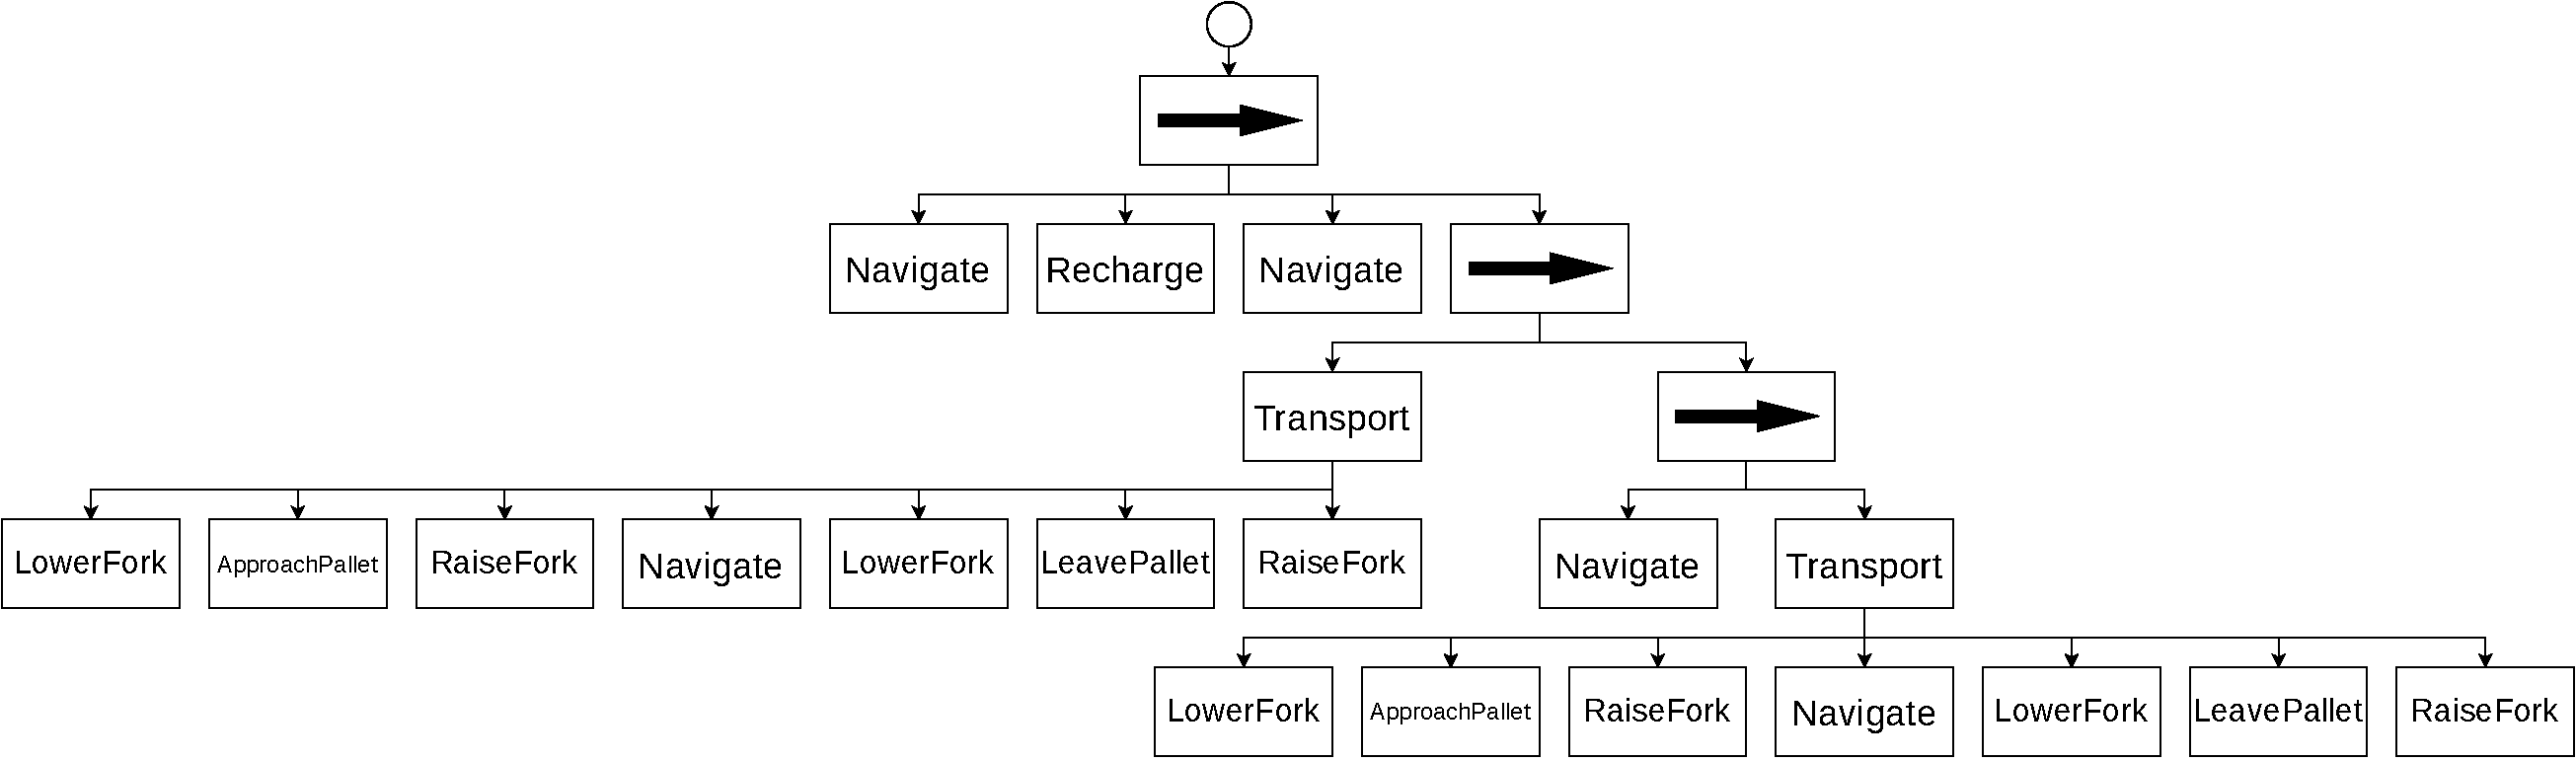
\includegraphics[width=\textwidth]{figures/example_bt.pdf}
        \caption[BT from SemReBot2 example]{A suitable BT for the plan generated in Example \ref{ex:task_controller}.}
        \label{fig:example_bt}
    \end{figure}
\end{example}

PlanSys2's action performer will tick the BT. Once the \verb|Navigate| BT node is ticked, it will make a call to Nav2's \verb|NavigateToPose| action server which then makes TARS move to the goal pose in the \verb|navigate| PDDL action.

Files \verb|domain.pddl| and \verb|problem.pddl| can be seen in Appendix \textcolor{red}{X}.

\section{Hardware requirements}
SemReBot2 is designed to run locally on a single GPU. We run it on a GPU with 12 GB memory, which is more than enough when loading Whisper Large with flash attention and Mistral 7B Instruct in 4-bit quantized size.